\documentclass[tikz,border=10pt]{standalone}
\usepackage{tikz}
\usetikzlibrary{shapes, arrows.meta, positioning, fit, calc}
\usepackage{soul}
\usepackage{textcomp}

% Define styles for nodes
\tikzset{
  level0/.style = {rectangle, draw=black, very thick, minimum width=3cm, minimum height=1cm, text centered, font=\sffamily\bfseries},
  level1/.style = {rectangle, rounded corners, draw=black, very thick, minimum width=1.5cm, minimum height=1cm, text centered, font=\sffamily\bfseries},
  level2/.style = {rectangle, draw=black, thick, minimum width=1.35cm, minimum height=1cm, text centered, font=\sffamily},
  level3/.style = {rectangle, rounded corners, draw=miamired, thick, font=\ttfamily, text=black, align=left, inner sep=2pt, minimum width=2cm, minimum height = .85cm}
}

% Define the 'miamired' color
\definecolor{miamired}{RGB}{200,16,46}

\begin{document}
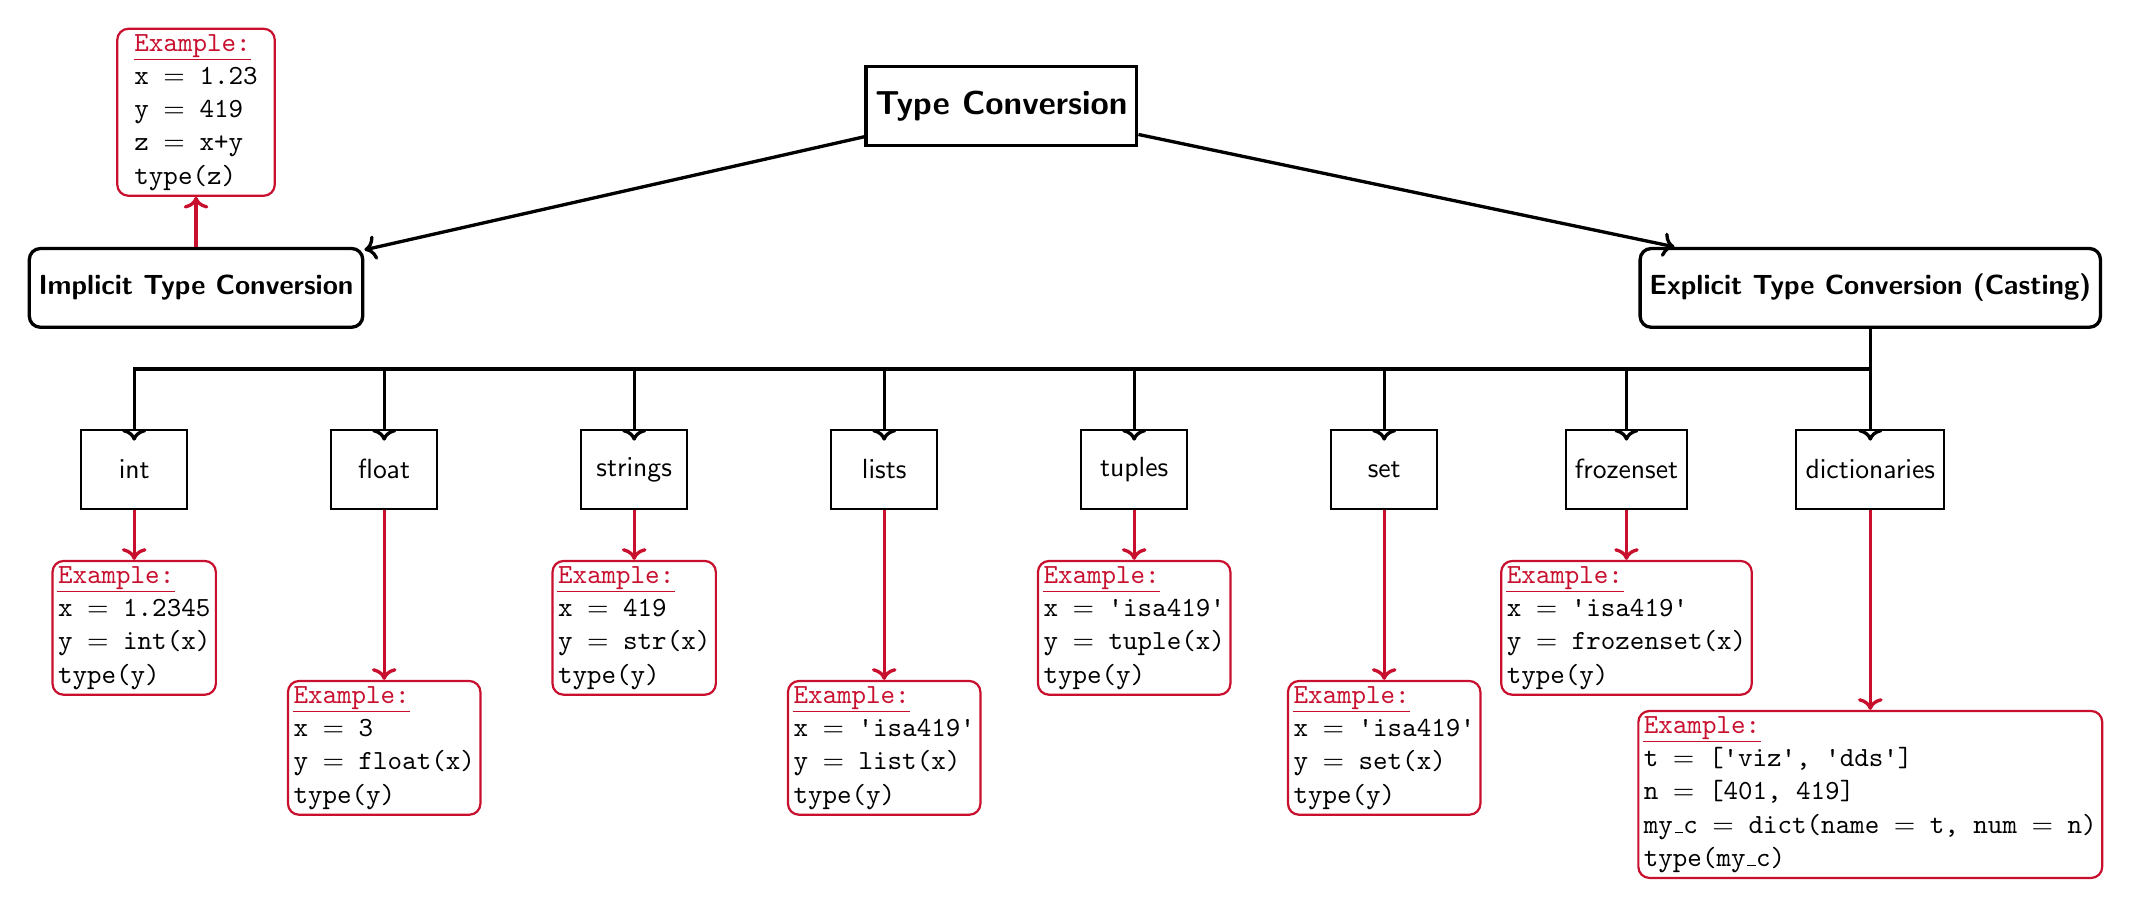
\begin{tikzpicture}

  % Level 0: Python - Data Types/Classes
  \node (type) [level0] {\large{Type Conversion}};

  % Level 1: None, Numbers, Sequences, Set types, Mappings, Callables/Modules/etc

  
  \node (implicit) [level1, below left=0.5in and 2.5in of type] {Implicit Type Conversion};

  \node (explicit) [level1, below right=0.5in and 2.5in of type] {Explicit Type Conversion (Casting)};

  % Level 2: Boxes under Numbers, Sequences, Set types, Mappings
  \node (dictionaries) [level2, below=0.5in of explicit] {dictionaries};
  \node (frozenset) [level2, below left=0.5in and -0.25in of explicit] {frozenset};
  \node (set) [level2,  below left=0.5in and 1in of explicit] {set};
  \node (tuples) [level2, below left=0.5in and 2.25in of explicit] {tuples};
  \node (lists) [level2, below left=0.5in and 3.5in of explicit] {lists};
  \node (strings) [level2, below left=0.5in and 4.75in of explicit] {strings};
  \node (float) [level2, below left=0.5in and 6.0in of explicit] {float};
  \node (int) [level2, below left=0.5in and 7.25in of explicit] {int};  
  
  % \node (complex) [level2, right=0.25in of float] {complex};

  % Level 3: Examples
  % \node (none_example) [level3, below=1.75in of none] {\textcolor{miamired}{\ul{Example:}}\\ x = None };

  \node(imp_example) [level3, above= 0.25in of implicit]{\textcolor{miamired}{\ul{Example:}}\\x $=$ 1.23 \\ y $=$ 419\\ z $=$ x+y \\ type(z)};

  \node (int_example) [level3, below=0.25in of int] {\textcolor{miamired}{\ul{Example:}}\\ x $=$ 1.2345 \\ y $=$ int(x) \\ type(y) };
  \node (float_example) [level3, below=0.85in of float] {\textcolor{miamired}{\ul{Example:}}\\ x $=$ 3 \\ y $=$ float(x) \\ type(y) };
  % \node (complex_example) [level3, below=0.25in of complex] {\textcolor{miamired}{\ul{Example:}}\\ x = 1+2j };

  \node (strings_example) [level3, below=0.25in of strings] {\textcolor{miamired}{\ul{Example:}}\\ x $=$ 419 \\ y $=$ str(x) \\ type(y)};
  \node (tuples_example) [level3, below=0.25in of tuples] {\textcolor{miamired}{\ul{Example:}}\\ x  $=$  \textquotesingle isa419\textquotesingle \\ y $=$ tuple(x) \\type(y) };
  \node (lists_example) [level3, below=0.85in of lists] {\textcolor{miamired}{\ul{Example:}}\\ x $=$ \textquotesingle isa419\textquotesingle \\ y $=$ list(x) \\type(y) };

  \node (set_example) [level3, below=0.85in of set] {\textcolor{miamired}{\ul{Example:}}\\ x $=$ \textquotesingle isa419\textquotesingle \\ y $=$ set(x) \\type(y)  };
  \node (frozenset_example) [level3, below=0.25in of frozenset] {\textcolor{miamired}{\ul{Example:}}\\ x $=$ \textquotesingle isa419\textquotesingle \\ y $=$ frozenset(x) \\type(y)  };

  \node (dictionaries_example) [level3, below=1in of dictionaries] {\textcolor{miamired}{\ul{Example:}}\\ t $=$ [\textquotesingle viz\textquotesingle, \textquotesingle dds\textquotesingle] \\ n $=$ [401, 419] \\ my\_c $=$ dict(name $=$ t, num $=$ n) \\ type(my\_c)};

  % Connect nodes with arrows
   \draw[->, very thick] (type) -- (implicit);
   \draw[->, very thick] (type) -- (explicit);
   
  % \draw[->, thick] (data_types) -- (none);
    \draw[-<, very thick] ($(explicit.south) + (0,-0.2in)$) -| ($(int.north)$) |- (int.north);
    \draw[-<, very thick] ($(explicit.south) + (0,-0.2in)$) -| ($(float.north) + (0,0.5cm)$) |- (float.north);
    \draw[-<, very thick] ($(explicit.south) + (0,-0.2in)$) -| ($(strings.north) + (0,0.5cm)$) |- (strings.north);
    \draw[-<, very thick] ($(explicit.south) + (0,-0.2in)$) -| ($(tuples.north) + (0,0.5cm)$) |- (tuples.north);
    \draw[-<, very thick] ($(explicit.south) + (0,-0.2in)$) -| ($(lists.north) + (0,0.5cm)$) |- (lists.north);
    \draw[-<, very thick] ($(explicit.south) + (0,-0.2in)$) -| ($(set.north) + (0,0.5cm)$) |- (set.north);
    \draw[-<, very thick] ($(explicit.south) + (0,-0.2in)$) -| ($(frozenset.north) + (0,0.5cm)$) |- (frozenset.north);
    \draw[-<, very thick] (explicit.south) -| ($(dictionaries.north) + (0,0.5cm)$) |- (dictionaries.north);


  \draw[->, miamired, very thick] (implicit) -- (imp_example);
  \draw[->, miamired, very thick] (dictionaries) -- (dictionaries_example);
  % \draw[->, miamired, very thick] (none) -- (none_example);
  \draw[->, miamired, very thick] (int) -- (int_example);
  \draw[->, miamired, very thick] (float) -- (float_example);
  % \draw[->, miamired, very thick] (complex) -- (complex_example);
  \draw[->, miamired, very thick] (strings) -- (strings_example);
  \draw[->, miamired, very thick] (tuples) -- (tuples_example);
  \draw[->, miamired, very thick] (lists) -- (lists_example);
  \draw[->, miamired, very thick] (set) -- (set_example);
  \draw[->, miamired, very thick] (frozenset) -- (frozenset_example);
\end{tikzpicture}
\end{document}
